\documentclass[a4paper]{article}

\usepackage[UTF8]{ctex}
\usepackage[a4paper,margin=1in]{geometry}
\usepackage{graphicx}
\usepackage{float}
\usepackage{longtable}
\usepackage{booktabs}
\usepackage{hyperref}
\usepackage{fancyhdr}
\usepackage{lastpage}
\usepackage{indentfirst}        % 首段缩进
\setlength{\parindent}{2em}     % 缩进2字符

\newcommand{\college}{中山大学计算机学院}
\newcommand{\projname}{软件工程课程项目}
\newcommand{\reporttitle}{LifeMaster系统建模报告}
\newcommand{\authorname}{刘昊、彭怡萱、马福泉、林炜东、刘贤彬、刘明宇}
\newcommand{\major}{软件工程}
\newcommand{\adviser}{郑贵峰}
\newcommand{\startdate}{2025年3月1日}
\newcommand{\labenddate}{2025年7月6日}
\newcommand{\labroom}{计算机学院}

\pagestyle{fancy}
\fancyhf{}
\fancyhead[L]{\kaishu \projname}
\fancyhead[C]{\kaishu \reporttitle}
\fancyhead[R]{\kaishu 项目团队}
\fancyfoot[C]{第 \thepage 页,共 \pageref{LastPage} 页}
\renewcommand{\headrulewidth}{0.4pt}
\renewcommand{\footrulewidth}{0pt}

\begin{document}

% 封面
\begin{titlepage}
    \centering
    
    
\includegraphics[width=12cm]{img/SYSULogo.png}

    \vspace{1em}
    {\Large \college \par}
    \vspace{1em}
    {\Large \kaishu \projname \par}
    \vspace{3em}

    {\fontsize{40pt}{42pt}\kaishu \selectfont \boldmath \reporttitle\par}
    \vspace*{\fill}

    \begin{center}
    {\Large
    \makebox[5em][s]{项目名称}:\underline{\makebox[15em][c]{\kaishu LifeMaster}}\\[1em]
    \makebox[5em][s]{组员姓名}:\underline{\makebox[15em][c]{\kaishu 刘昊、彭怡萱、马福泉}}\\[0.5em]
    \makebox[5em][s]{}:\underline{\makebox[15em][c]{\kaishu 林炜东、刘贤彬、刘明宇}}\\[1em]
    \makebox[5em][s]{专业}:\underline{\makebox[15em][c]{\kaishu \major}}\\[1em]
    \makebox[5em][s]{课程教师}:\underline{\makebox[15em][c]{\kaishu \adviser}}\\[1em]
    \makebox[5em][s]{起始日期}:\underline{\makebox[15em][c]{\kaishu \startdate}}\\[1em]
    \makebox[5em][s]{结束日期}:\underline{\makebox[15em][c]{\kaishu \labenddate}}\\[1em]
    \makebox[5em][s]{学院}:\underline{\makebox[15em][c]{\kaishu \labroom}}
    }
    \end{center}

    \vspace*{\fill}
\end{titlepage}

% 目录
\tableofcontents
\newpage

\section{系统概述}

LifeMaster是一个集成待办事项管理、记账管理和手账管理功能的个人生活管理系统。本报告通过UML建模图形系统地描述了系统的结构、行为和交互关系,包括类图、顺序图、用例图、活动图和状态图等多个维度的建模分析。

\subsection{建模目的}

通过UML建模,我们可以:

\begin{itemize}
    \item \textbf{结构化设计}:清晰地定义系统的静态结构和动态行为
    \item \textbf{需求分析}:准确理解和表达系统的功能需求
    \item \textbf{沟通工具}:为开发团队提供统一的理解基础
    \item \textbf{设计验证}:确保系统设计的完整性和一致性
\end{itemize}

\section{类图(UML)}

\subsection{类图概述}

类图描述了LifeMaster系统中的核心实体及其相互关系。系统主要包含用户管理、任务管理、记账管理和手账管理四个核心模块。

\begin{figure}[H]
\centering
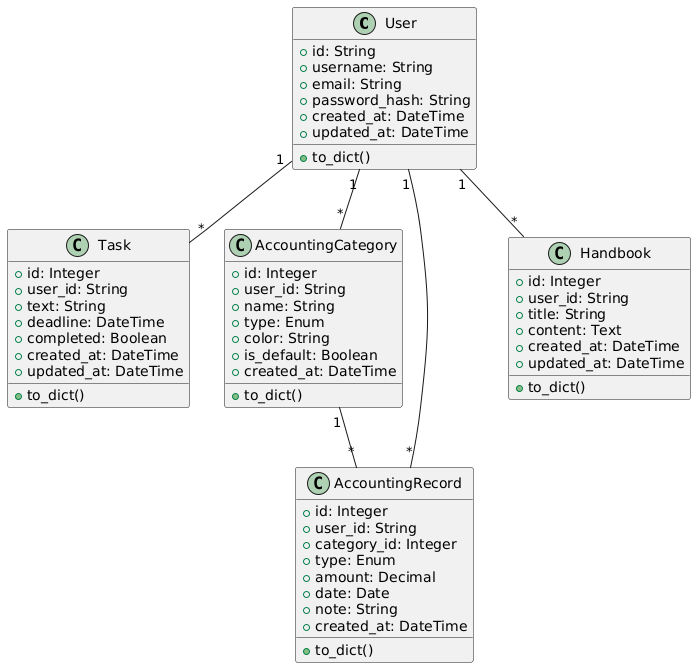
\includegraphics[width=0.9\textwidth]{img/class_diagram.png}
\caption{LifeMaster系统类图}
\end{figure}

\subsection{核心类说明}

\subsubsection{User类(用户类)}

User类是系统的核心用户实体,包含用户的基本信息和权限管理。

\textbf{主要属性:}
\begin{itemize}
    \item \texttt{id: String} - 用户唯一标识符
    \item \texttt{username: String} - 用户名
    \item \texttt{email: String} - 电子邮箱地址
    \item \texttt{password\_hash: String} - 密码哈希值
    \item \texttt{created\_at: DateTime} - 账户创建时间
    \item \texttt{updated\_at: DateTime} - 最后更新时间
\end{itemize}

\textbf{主要方法:}
\begin{itemize}
    \item \texttt{login(username, password): Boolean} - 用户登录验证
    \item \texttt{logout(): void} - 用户登出
    \item \texttt{updateProfile(userInfo): Boolean} - 更新用户信息
    \item \texttt{changePassword(oldPass, newPass): Boolean} - 修改密码
\end{itemize}

\subsubsection{Task类(任务类)}

Task类管理用户的待办事项,支持任务的创建、编辑、删除和状态管理。

\textbf{主要属性:}
\begin{itemize}
    \item \texttt{id: Integer} - 任务唯一标识符
    \item \texttt{user\_id: String} - 所属用户ID
    \item \texttt{title: String} - 任务标题
    \item \texttt{description: String} - 任务描述
    \item \texttt{deadline: DateTime} - 截止时间
    \item \texttt{status: TaskStatus} - 任务状态(待完成/已完成/已过期)
    \item \texttt{priority: Priority} - 优先级(高/中/低)
    \item \texttt{created\_at: DateTime} - 创建时间
    \item \texttt{updated\_at: DateTime} - 更新时间
\end{itemize}

\textbf{主要方法:}
\begin{itemize}
    \item \texttt{create(taskInfo): Task} - 创建新任务
    \item \texttt{update(taskInfo): Boolean} - 更新任务信息
    \item \texttt{delete(): Boolean} - 删除任务
    \item \texttt{markCompleted(): Boolean} - 标记任务为已完成
    \item \texttt{setDeadline(date): Boolean} - 设置截止时间
\end{itemize}

\subsubsection{AccountingCategory类(记账分类类)}

AccountingCategory类管理记账的分类信息,为记账记录提供分类支持。

\textbf{主要属性:}
\begin{itemize}
    \item \texttt{id: Integer} - 分类唯一标识符
    \item \texttt{user\_id: String} - 所属用户ID
    \item \texttt{name: String} - 分类名称
    \item \texttt{type: CategoryType} - 分类类型(收入/支出)
    \item \texttt{color: String} - 分类颜色标识
    \item \texttt{icon: String} - 分类图标
    \item \texttt{created\_at: DateTime} - 创建时间
    \item \texttt{updated\_at: DateTime} - 更新时间
\end{itemize}

\textbf{主要方法:}
\begin{itemize}
    \item \texttt{create(categoryInfo): AccountingCategory} - 创建新分类
    \item \texttt{update(categoryInfo): Boolean} - 更新分类信息
    \item \texttt{delete(): Boolean} - 删除分类
    \item \texttt{getRecordsByCategory(): List<AccountingRecord>} - 获取该分类下的记录
\end{itemize}

\subsubsection{AccountingRecord类(记账记录类)}

AccountingRecord类管理具体的收支记录信息。

\textbf{主要属性:}
\begin{itemize}
    \item \texttt{id: Integer} - 记录唯一标识符
    \item \texttt{user\_id: String} - 所属用户ID
    \item \texttt{category\_id: Integer} - 所属分类ID
    \item \texttt{amount: Decimal} - 金额
    \item \texttt{description: String} - 记录描述
    \item \texttt{date: Date} - 记录日期
    \item \texttt{created\_at: DateTime} - 创建时间
    \item \texttt{updated\_at: DateTime} - 更新时间
\end{itemize}

\textbf{主要方法:}
\begin{itemize}
    \item \texttt{create(recordInfo): AccountingRecord} - 创建记账记录
    \item \texttt{update(recordInfo): Boolean} - 更新记录信息
    \item \texttt{delete(): Boolean} - 删除记录
    \item \texttt{getStatistics(period): Statistics} - 获取统计信息
\end{itemize}

\subsubsection{Handbook类(手账类)}

Handbook类管理用户的手账内容,支持文本、图片等多媒体内容。

\textbf{主要属性:}
\begin{itemize}
    \item \texttt{id: Integer} - 手账唯一标识符
    \item \texttt{user\_id: String} - 所属用户ID
    \item \texttt{title: String} - 手账标题
    \item \texttt{content: Text} - 手账内容
    \item \texttt{images: String} - 图片路径列表
    \item \texttt{tags: String} - 标签列表
    \item \texttt{mood: Integer} - 心情评分(1-5)
    \item \texttt{date: Date} - 手账日期
    \item \texttt{created\_at: DateTime} - 创建时间
    \item \texttt{updated\_at: DateTime} - 更新时间
\end{itemize}

\textbf{主要方法:}
\begin{itemize}
    \item \texttt{create(handbookInfo): Handbook} - 创建手账
    \item \texttt{update(handbookInfo): Boolean} - 更新手账内容
    \item \texttt{delete(): Boolean} - 删除手账
    \item \texttt{addImage(imagePath): Boolean} - 添加图片
    \item \texttt{setMood(moodLevel): Boolean} - 设置心情评分
\end{itemize}

\subsection{类之间的关系}

\begin{itemize}
    \item \textbf{User与Task}:一对多关系,一个用户可以有多个任务
    \item \textbf{User与AccountingCategory}:一对多关系,一个用户可以创建多个记账分类
    \item \textbf{User与AccountingRecord}:一对多关系,一个用户可以有多个记账记录
    \item \textbf{User与Handbook}:一对多关系,一个用户可以创建多个手账
    \item \textbf{AccountingCategory与AccountingRecord}:一对多关系,一个分类可以包含多个记录
\end{itemize}

\section{顺序图(UML)}

顺序图描述了系统中各个对象之间的时序交互过程。以下是LifeMaster系统的关键业务流程顺序图。

\subsection{用户登录流程}

\begin{figure}[H]
\centering
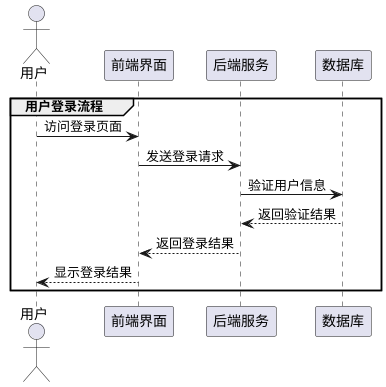
\includegraphics[width=0.9\textwidth]{img/sequence_diagram1.png}
\caption{用户登录流程顺序图}
\end{figure}

\textbf{流程说明:}

\begin{enumerate}
    \item 用户访问登录页面,前端显示登录界面
    \item 用户输入用户名和密码,点击登录按钮
    \item 前端发送登录请求到后端API
    \item 后端接收请求,查询数据库验证用户信息
    \item 数据库返回用户验证结果
    \item 如果验证成功,后端生成JWT token
    \item 后端将token返回给前端
    \item 前端接收token,存储到本地存储
    \item 前端显示登录成功消息并跳转到主页面
\end{enumerate}

\subsection{财务管理流程}

\subsubsection{记账分类管理}

\begin{figure}[H]
\centering
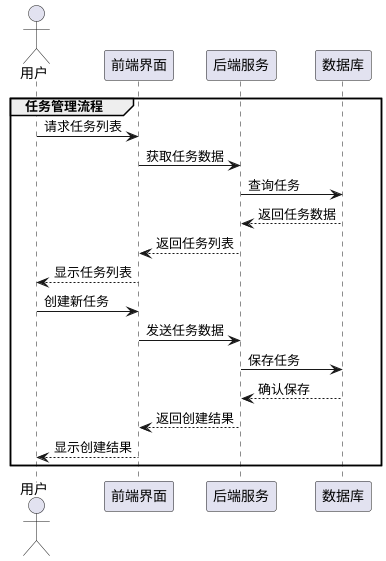
\includegraphics[width=0.9\textwidth]{img/sequence_diagram2.png}
\caption{记账分类管理顺序图}
\end{figure}

\textbf{流程说明:}

\begin{enumerate}
    \item 用户点击"分类管理"按钮
    \item 前端发送获取分类列表的请求
    \item 后端从数据库查询用户的所有分类
    \item 数据库返回分类数据列表
    \item 后端处理数据并返回给前端
    \item 前端接收数据并渲染分类列表界面
    \item 用户可以查看、编辑或删除分类
\end{enumerate}

\subsubsection{记账记录管理}

\begin{figure}[H]
\centering
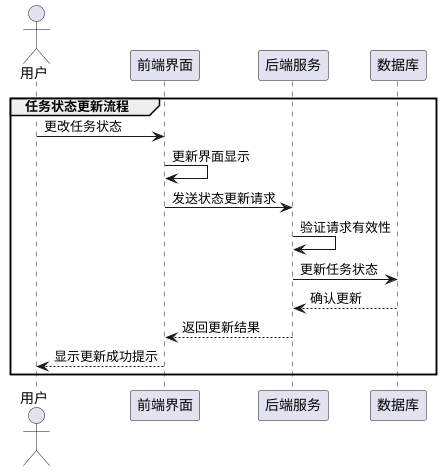
\includegraphics[width=0.9\textwidth]{img/sequence_diagram3.png}
\caption{记账记录管理顺序图}
\end{figure}

\textbf{流程说明:}

\begin{enumerate}
    \item 用户填写收支记录表单(金额、分类、描述等)
    \item 前端进行表单数据验证(必填项、格式检查)
    \item 验证通过后,前端提交记录数据到后端
    \item 后端接收数据,执行业务逻辑验证
    \item 后端将验证通过的数据存入数据库
    \item 数据库确认存储完成,返回操作结果
    \item 后端将操作结果返回给前端
    \item 前端显示操作成功消息,更新界面
\end{enumerate}

\subsubsection{账务统计分析}

\begin{figure}[H]
\centering
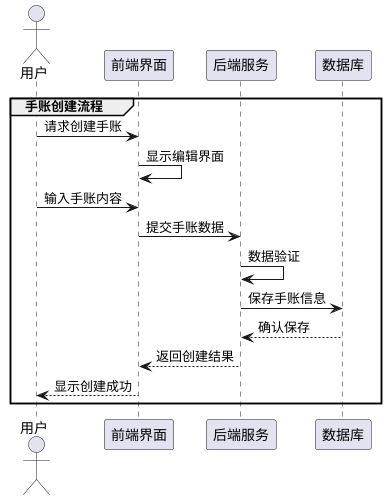
\includegraphics[width=0.9\textwidth]{img/sequence_diagram4.png}
\caption{账务统计分析顺序图}
\end{figure}

\textbf{流程说明:}

\begin{enumerate}
    \item 用户选择查看财务报表
    \item 前端发送统计数据请求(指定时间范围)
    \item 后端执行数据库聚合查询操作
    \item 数据库返回统计分析结果
    \item 后端处理统计数据,计算各项指标
    \item 后端将处理后的数据返回前端
    \item 前端使用Chart.js生成可视化图表
    \item 向用户展示包含图表的财务报表
\end{enumerate}

\subsection{手账创建流程}

手账创建是用户记录生活的重要功能,支持文本、图片和心情记录。

\textbf{流程说明:}

\begin{enumerate}
    \item 用户点击"新建手账"按钮
    \item 前端显示手账编辑界面
    \item 用户输入手账标题、内容、选择心情等
    \item 用户可选择上传图片文件
    \item 前端验证输入数据的完整性
    \item 前端提交手账数据到后端API
    \item 后端验证数据格式和权限
    \item 后端将手账数据保存到数据库
    \item 数据库确认保存成功
    \item 后端返回创建成功的响应
    \item 前端显示创建成功提示并刷新列表
\end{enumerate}

\subsection{任务状态更新}

任务状态更新是高频操作,需要保证界面响应性和数据一致性。

\textbf{流程说明:}

\begin{enumerate}
    \item 用户点击任务状态切换按钮(如完成按钮)
    \item 前端立即更新界面显示(乐观更新)
    \item 前端发送状态更新请求到后端
    \item 后端验证请求的合法性和权限
    \item 后端更新数据库中的任务状态
    \item 数据库确认更新操作完成
    \item 后端返回更新结果到前端
    \item 如果更新失败,前端回滚界面状态
    \item 前端显示相应的成功或失败提示
\end{enumerate}

\section{用例图(UML)}

用例图描述了系统的功能需求以及各类用户与系统的交互关系。

\begin{figure}[H]
\centering
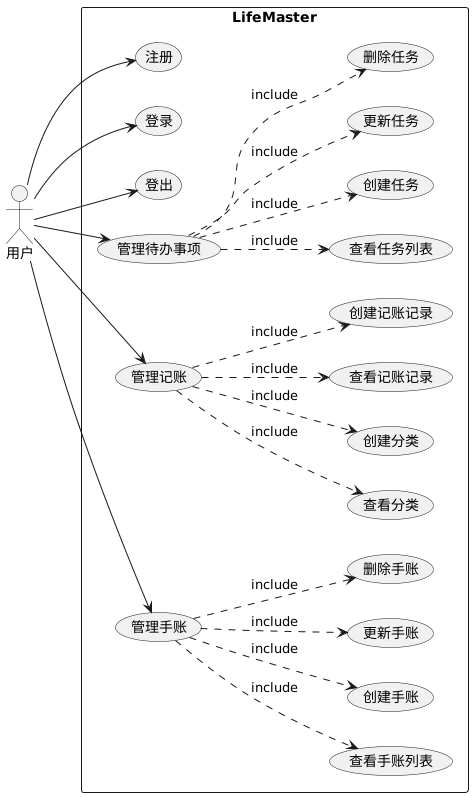
\includegraphics[width=0.9\textwidth]{img/use_case_diagram.png}
\caption{LifeMaster系统用例图}
\end{figure}

\subsection{主要用例说明}

\subsubsection{用户管理用例}

\begin{itemize}
    \item \textbf{用户注册}:新用户创建账户
    \item \textbf{用户登录}:已注册用户通过凭证访问系统
    \item \textbf{用户登出}:结束当前会话
    \item \textbf{修改个人信息}:更新用户基本信息
    \item \textbf{修改密码}:变更登录密码
\end{itemize}

\subsubsection{任务管理用例}

\begin{itemize}
    \item \textbf{查看任务列表}:显示用户的所有任务
    \item \textbf{创建任务}:添加新的待办事项
    \item \textbf{编辑任务}:修改任务内容、截止时间等
    \item \textbf{删除任务}:移除不需要的任务
    \item \textbf{标记任务完成}:更新任务状态
    \item \textbf{设置任务优先级}:调整任务的重要程度
\end{itemize}

\subsubsection{记账管理用例}

\begin{itemize}
    \item \textbf{查看记账记录}:浏览历史收支记录
    \item \textbf{添加收支记录}:记录新的收入或支出
    \item \textbf{编辑记录}:修改已有的记账信息
    \item \textbf{删除记录}:移除错误的记录
    \item \textbf{管理分类}:创建、编辑、删除记账分类
    \item \textbf{查看统计报表}:分析收支情况和趋势
    \item \textbf{导出数据}:将记账数据导出为文件
\end{itemize}

\subsubsection{手账管理用例}

\begin{itemize}
    \item \textbf{查看手账列表}:浏览所有手账记录
    \item \textbf{创建手账}:写新的日记或笔记
    \item \textbf{编辑手账}:修改手账内容
    \item \textbf{删除手账}:移除不需要的手账
    \item \textbf{上传图片}:为手账添加图片内容
    \item \textbf{设置心情}:记录当天的心情状态
    \item \textbf{添加标签}:为手账添加分类标签
\end{itemize}

\subsection{用例关系}

\begin{itemize}
    \item \textbf{包含关系}:用户登录是所有功能用例的前提条件
    \item \textbf{扩展关系}:设置提醒是创建任务的可选扩展
    \item \textbf{泛化关系}:添加收入记录和添加支出记录都是添加记录的特化
\end{itemize}

\section{活动图(UML)}

活动图描述了系统中主要业务流程的控制流和活动序列。

\begin{figure}[H]
\centering
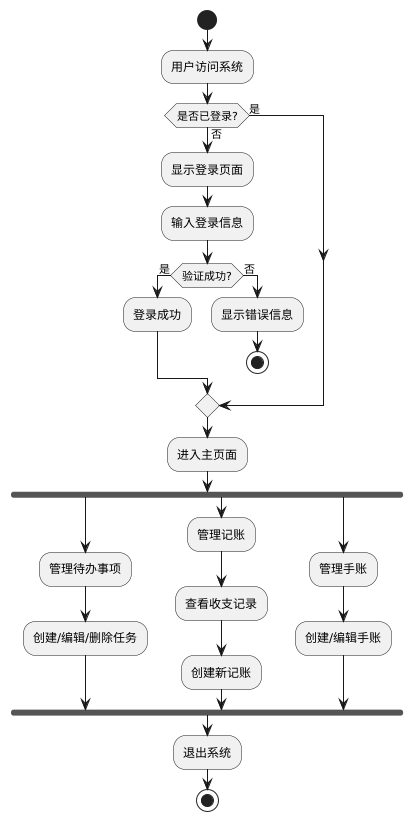
\includegraphics[width=0.6\textwidth]{img/activity_diagram.png}
\caption{LifeMaster系统主要活动流程图}
\end{figure}

\subsection{活动流程分解}

\subsubsection{步骤1:用户访问系统}

\textbf{初始节点:}用户打开应用或网页,触发系统访问。

\begin{itemize}
    \item 系统检查用户设备和浏览器兼容性
    \item 加载必要的静态资源(CSS、JavaScript等)
    \item 初始化用户界面框架
    \item 检查本地存储中的用户认证信息
\end{itemize}

\subsubsection{步骤2:登录验证}

\textbf{判断是否已登录:}

\begin{itemize}
    \item \textbf{是} → 验证token有效性,直接跳转至主页面
    \item \textbf{否} → 显示登录页面,要求用户输入凭证
\end{itemize}

\textbf{验证登录信息:}

\begin{itemize}
    \item \textbf{成功} → 生成新的访问token,进入主页面
    \item \textbf{失败} → 显示具体错误信息(如"用户名不存在"、"密码错误"等)
    \item 如果连续失败超过3次,触发账户临时锁定机制
    \item 提供"忘记密码"选项,引导用户重置密码
\end{itemize}

\subsubsection{步骤3:主页面功能操作}

用户登录成功后,可以执行以下操作(并行执行):

\textbf{管理待办事项:}
\begin{itemize}
    \item 查看任务概览:显示今日任务、即将到期任务等
    \item 创建任务:填写任务信息(标题、描述、截止时间、优先级)
    \item 编辑任务:修改现有任务的任何属性
    \item 删除任务:移除不需要的任务(需确认操作)
    \item 批量操作:支持批量标记完成、删除等操作
\end{itemize}

\textbf{管理记账:}
\begin{itemize}
    \item 查看记录:按时间、分类、金额等条件筛选查看
    \item 添加记录:选择分类、输入金额、添加备注信息
    \item 统计分析:查看月度、季度、年度的收支统计
    \item 分类管理:自定义收入和支出的分类体系
    \item 预算设置:为不同分类设置月度预算限额
\end{itemize}

\textbf{手账管理:}
\begin{itemize}
    \item 浏览手账:按日期、标签、心情等方式查看
    \item 创建手账:写日记、添加图片、标记心情、设置标签
    \item 编辑手账:修改已有的手账内容和属性
    \item 搜索功能:根据关键词搜索手账内容
    \item 导出功能:将手账内容导出为PDF或其他格式
\end{itemize}

\subsubsection{步骤4:退出系统}

\textbf{正常退出流程:}
\begin{itemize}
    \item 用户主动选择退出操作
    \item 系统保存所有未提交的更改
    \item 清理客户端缓存和临时数据
    \item 注销服务器端的用户会话
    \item 清除本地存储的认证信息
    \item 返回登录页面或欢迎页面
\end{itemize}

\textbf{异常退出处理:}
\begin{itemize}
    \item 会话超时自动退出
    \item 检测到异常登录时强制退出
    \item 网络中断时的客户端状态保护
\end{itemize}

\section{状态图(UML)}

状态图描述了系统中关键对象在其生命周期内状态的变化过程。

\begin{figure}[H]
\centering
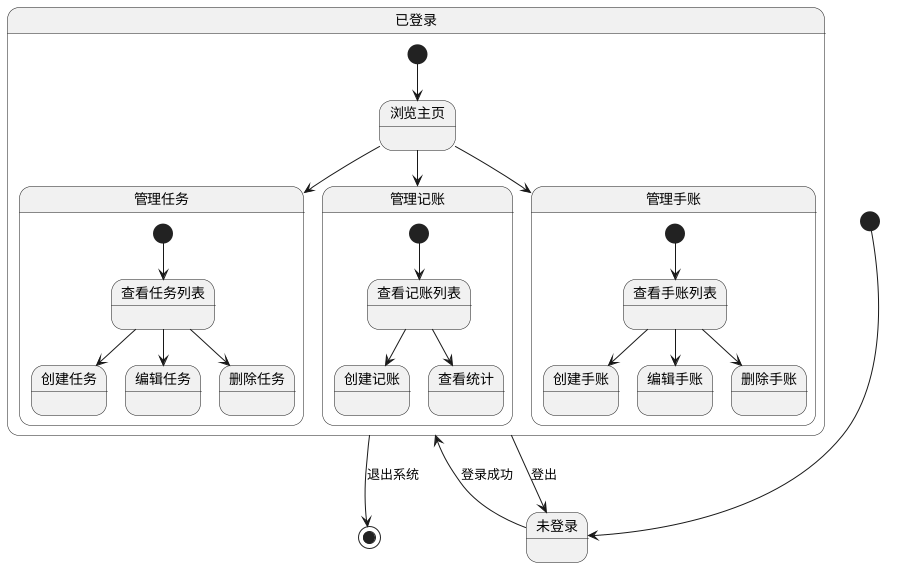
\includegraphics[width=0.9\textwidth]{img/state_diagram.png}
\caption{用户会话状态图}
\end{figure}

\subsection{核心状态与转换}

\subsubsection{(1)未登录(初始状态)}

\textbf{触发条件:}
\begin{itemize}
    \item 用户首次访问系统
    \item 用户主动退出系统
    \item 会话token过期
    \item 系统检测到安全异常强制登出
\end{itemize}

\textbf{允许操作:}
\begin{itemize}
    \item 查看登录页面
    \item 尝试登录验证
    \item 访问用户注册功能
    \item 查看忘记密码功能
    \item 浏览系统介绍页面(如果有)
\end{itemize}

\textbf{状态特征:}
\begin{itemize}
    \item 无法访问任何受保护的功能
    \item 不保存任何用户个人数据
    \item 只能进行公开的、不涉及个人信息的操作
\end{itemize}

\subsubsection{(2)已登录(核心状态)}

\textbf{进入条件:}
\begin{itemize}
    \item 用户成功通过登录验证
    \item 系统验证用户凭证有效
    \item 生成有效的访问token
\end{itemize}

\textbf{子状态详解:}

用户在已登录状态下可以自由切换以下功能模块:

\textbf{管理任务子状态:}
\begin{itemize}
    \item \textbf{查看任务列表}:显示所有任务的概览视图
    \item \textbf{创建任务}:进入任务创建模式,填写必要信息
    \item \textbf{编辑任务}:修改选定任务的属性和内容
    \item \textbf{删除任务}:移除不需要的任务项目
\end{itemize}

\textbf{管理记录(记账)子状态:}
\begin{itemize}
    \item \textbf{查看记录列表}:浏览历史收支记录
    \item \textbf{创建记录}:添加新的收入或支出记录
    \item \textbf{编辑记录}:修改已有记录的详细信息
    \item \textbf{查看统计}:生成和展示财务分析报表
    \item \textbf{管理分类}:维护收支分类体系
\end{itemize}

\textbf{管理手账子状态:}
\begin{itemize}
    \item \textbf{查看手账列表}:浏览所有手账记录
    \item \textbf{创建手账}:写新的日记或笔记内容
    \item \textbf{编辑手账}:修改现有手账的内容和属性
    \item \textbf{删除手账}:移除不需要的手账记录
\end{itemize}

\textbf{状态转换条件:}
\begin{itemize}
    \item 用户通过导航菜单选择不同功能
    \item 通过快捷操作直接跳转到特定功能
    \item 系统根据用户行为自动切换相关状态
\end{itemize}

\subsubsection{(3)退出系统(终止状态)}

\textbf{触发条件:}
\begin{itemize}
    \item 用户主动选择退出登录
    \item 系统检测到会话超时
    \item 管理员强制用户下线
    \item 检测到账户安全异常
\end{itemize}

\textbf{处理流程:}
\begin{itemize}
    \item 保存用户当前的工作状态
    \item 清理客户端的敏感数据
    \item 注销服务器端的用户会话
    \item 记录用户退出日志
\end{itemize}

\textbf{结果状态:}
\begin{itemize}
    \item 返回"未登录"状态
    \item 需要重新进行身份验证才能访问系统功能
    \item 清除所有本地缓存的用户数据
\end{itemize}

\subsection{状态转换的触发事件}

\begin{itemize}
    \item \textbf{登录成功事件}:从"未登录"转换到"已登录"
    \item \textbf{退出事件}:从"已登录"转换到"未登录"
    \item \textbf{功能切换事件}:在"已登录"状态的各子状态间转换
    \item \textbf{会话超时事件}:自动从"已登录"转换到"未登录"
    \item \textbf{安全异常事件}:强制从任何状态转换到"未登录"
\end{itemize}

\section{建模总结}

\subsection{建模成果}

通过UML建模,我们完成了LifeMaster系统的全面设计分析:

\begin{itemize}
    \item \textbf{类图}:明确定义了系统的核心实体和它们之间的关系
    \item \textbf{顺序图}:详细描述了关键业务流程的时序交互
    \item \textbf{用例图}:全面梳理了系统的功能需求和用户交互
    \item \textbf{活动图}:清晰展现了业务流程的控制逻辑
    \item \textbf{状态图}:准确描述了用户会话的状态变迁
\end{itemize}

\subsection{设计验证}

通过建模过程,我们验证了系统设计的:

\begin{itemize}
    \item \textbf{完整性}:所有核心功能都有对应的建模描述
    \item \textbf{一致性}:各个建模图之间保持逻辑一致
    \item \textbf{可追溯性}:需求与设计之间建立了清晰的映射关系
    \item \textbf{可实现性}:建模设计考虑了技术实现的可行性
\end{itemize}

\subsection{指导意义}

本建模报告为LifeMaster系统的后续开发提供了:

\begin{itemize}
    \item \textbf{开发指南}:为程序员提供清晰的实现指导
    \item \textbf{测试依据}:为测试用例设计提供参考标准
    \item \textbf{维护支持}:为系统维护和扩展提供文档支撑
    \item \textbf{沟通工具}:为团队协作提供统一的理解基础
\end{itemize}

通过系统性的UML建模,我们确保了LifeMaster系统设计的科学性和规范性,为项目的成功实施奠定了坚实的基础。

\label{LastPage}
\end{document}
